%!TEX root = latex.tex

\subsection{Context}

\begin{frame}{Dimensions of a Document}
  \begin{onlyenv}<presentation:1| article:0>
    \begin{center}
      Content is the meaning of a document.
    \end{center}
  \end{onlyenv}
  \begin{onlyenv}<presentation:2| article:0>
    \begin{description}
      \item[\textnormal{\color{black}Content}] is the \emph{meaning} of a document.
      \item[\textnormal{\color{black}Structure}] is the \emph{outline }  of a document.
      \uncover<3>{\item Foo}
    \end{description}
  \end{onlyenv}
  \begin{onlyenv}<3>
    \begin{description}
      \item[Content] is the \alert{meaning}  of a document.
      \item[Structure] is the \alert{outline}  of a document.
      \item[Form] is the \alert{apperance} of a document.
    \end{description}
  \end{onlyenv}
\end{frame}

\begin{frame}{Structure vs. Form}
  \begin{Beispiele}[Structure]
    \begin{itemize}
      \item heading
      \item grouping
      \item listing
    \end{itemize}
  \end{Beispiele}

  \xxx

  \begin{Beispiele}[Form]
    \begin{itemize}
      \item 13{,}37~cm wide coloured box
      \item 0{,}6~cm indentation
      \item bullet $\blacktriangleright$ at beginning of the column
    \end{itemize}
  \end{Beispiele}
\end{frame}

\begin{frame}[fragile]{Markdown Languages}
  \newcommand{\entry}[2]{\draw[maincolor, thick] (-.2,#1) -- (.2,#1) node[right] {\color{black}#2};}
  \hskip 8ex\begin{tikzpicture}
    \draw[maincolor, thick] (0,0) node[below] {\textbf{Form}} edge[<->] (0,6);
    \draw[maincolor] (0,6) node[above] {\textbf{Struktur}};
    \entry{.5}{Pixel graphics e.\,g. Paint};
    \entry{1}{Vector graphics e.\,g. Inkscape};
    \entry{1.5}{PDF};
    \entry{2.5}{\TeX};
    \entry{3}{DTP-Tools  e.\,g. Scribus};
    \entry{3.5}{Office Word, Writer, \ldots};
    \entry{4}{\textcolor{examplecolor}{\LaTeX}};
    \entry{4.75}{HTML};
    \entry{5.5}{Outliner};
  \end{tikzpicture}
\end{frame}

\begin{frame}{\LaTeX\ vs. Office Word}
  \begin{center}
    \begin{tikzpicture}[thick]
      \draw[->] (0,0) -- node[below] {Document size and -complexity} (8,0);
      \draw[->] (0,0) -- node[rotate=90, above] {Effort and time requirement} (0,6);
      \begin{scope}[
          every node/.style={font=\Large},
        ]
        \draw[alertedcolor, domain=0:3.68965] plot (\x, {exp(\x+.5)/12 + .5});
        \path[alertedcolor, domain=0:3.3] plot (\x, {exp(\x+.5)/12 + .5}) node[above left] {Office Word};
        \pause
        \draw[dashed, maincolor] (0,5.5) -- node[above,near end] {hopeless} (8,5.5);
        \pause
        \draw[examplecolor, domain=0:8] plot (\x, {\x^2/25 + 1.5});
        \path[examplecolor, domain=0:6] plot (\x, {\x^2/25 + 1.5}) node[below right] {\LaTeX};
      \end{scope}
    \end{tikzpicture}
  \end{center}
\end{frame}

\subsection{\LaTeX-Documents}

\begin{frame}[fragile]{A \LaTeX-Document}
  \begin{itemize}
    \item<1-> are pure \alert{text files} with \alert{content}
    \item<2-> also contain \alert{structure} of the content
    \item<3-> typesetting is done by \LaTeX\  \alert{separately}
  \end{itemize}

  \xxx
  
  \begin{center}
    \begin{tikzpicture}[
        shorten <=5pt,
        shorten >=5pt
      ]
      \matrix[column sep=3em] {
        \node[text width=6em] (source) {
          \only<1>{\lstinputlisting[
              basicstyle=\ttfamily\fontsize{4}{4}\selectfont 
            ]{demo/exampleContent.txt}}
          \only<2->{\lstinputlisting[
              basicstyle=\ttfamily\fontsize{4}{4}\selectfont,
              linerange={1-1,12-27}
            ]{demo/example.tex}}
        };
        &
        \visible<3->{\node[inner sep=0pt] (latex)
          {\rmfamily\Large\bfseries\LaTeX};}
        &
        \visible<3->{\node[draw=maincolor, thick] (pdf) {
          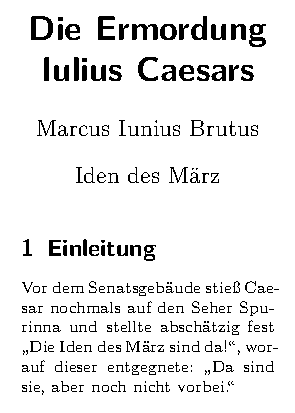
\includegraphics[width=6em]{demo/example.pdf}
        };}\\
        \node {\shortstack{Content \visible<2->{\&\\ Structure}}};
        & & 
        \visible<3->{\node {\shortstack{typeset\\Document}};}\\
      };
      \visible<3->{\path[very thick, ->]
        (source) edge (latex)
        (latex) edge (pdf);}
    \end{tikzpicture}
  \end{center}
\end{frame}
